\section{Environment}
\label{sec:environment}

\subsection{Structure}
OOP
Modules
Separation of concerns

\subsection{Team builder}

\subsection{Team parser}

\subsection{Gymnasium environment}
The custom environment was implemented using a custom Gymnasium \cite{Gymnasium} environment \cite{GymnasiumCustomEnv}. 
The \lstinline|BattleEnv| class extends the Gymnasium \lstinline|Env| class and implements the abstract methods within.
There are 4 requirements for using the \lstinline|Env| class. The custom environment needs to define its own:

\begin{itemize}
    \item Action space
    \item Observation space
    \item Step function
    \item Reset function
\end{itemize}

\subsubsection{Action space}
The action space is a normalized representation of the actions an agent can perform. In the domain of Pokemon this presented 
an interesting challenge as the amount of actions change depending on the configuration of a Pokemon and team. When using
reinforcement learning it is important for the action space to be static in order to be compatible with PyTorch's DQN model.
For this reason the action space is then defined as a discrete space at the maximum size possible within the bounds of the domain.
This accounts for maximum 6 different switches per team, maximum 4 moves per Pokemon and maximum 2 targets per move, thus 
resulting in an action space of size 14 (see listing \ref{lst:action-space-def}).

\begin{lstlisting}[basicstyle=\fontsize{10}{10}\selectfont\ttfamily,language=Python,caption={The defined action space.},label=lst:action-space-def,breaklines]
MAX_PLAYER_SWITCH_OPTIONS = 6
MAX_PLAYER_MOVES = 4
MAX_MOVE_TARGETS = 2
self.action_space = gym.spaces.Discrete(MAX_PLAYER_MOVES * MAX_MOVE_TARGETS + MAX_PLAYER_SWITCH_OPTIONS)
\end{lstlisting}

At this stage the action space would allow potentially illegal actions to be taken by the agent. To counteract this it was 
necessary to implement an action mask (see listing \ref{lst:action-mask}). The mask is an array of equal size to the action space
consisting of booleans. The state is then iterated through to determine what actions are currently legal. If an action is legal
the corresponding mask index will be set to \lstinline|True|. When the agent goes to select an action it will first request 
a mask and then limit its options accordingly.

\begin{lstlisting}[basicstyle=\fontsize{10}{10}\selectfont\ttfamily,language=Python,caption={The action mask that makes sure only valid actions are being evaluated.},label=lst:action-mask,breaklines]
def get_action_mask(self, side: Side) -> np.ndarray:
    active_pokemon = self.state.battle_field[0] if side == 'player' else self.state.battle_field[1]
    team = self.state.player_team if side == 'player' else self.state.opponent_team

    mask = np.zeros(self.action_space_size, dtype=np.bool)

    if active_pokemon.is_fainted():
        for i, pkm in enumerate(team):
            switch_index = 8 + i  # 8 is the beginning of team switch options
            if not pkm.is_fainted() and not pkm.active:
                mask[switch_index] = True
        return mask

    for i, move in enumerate(active_pokemon.moves):
        if move.current_pp > 0:  # Only allow moves with PP remaining
            mask[i * 2] = True  # Target 0
            mask[i * 2 + 1] = True  # Target 1

    for i, pkm in enumerate(team):
        switch_index = 8 + i  # 8 is the beginning of team switch options
        if not pkm.is_fainted() and not pkm.active:
            mask[switch_index] = True

    return mask
\end{lstlisting}

To actually execute an action selected by the agent a map was created. The map is defined as a \lstinline|Dict| with the keys
0-13 matching the indices of the action space. Each key then corresponds to a function from the \lstinline|BattleActions|
class defined in the Pokemon domain (see section \ref{subsec:pokemon-domain}). 

\subsubsection{Observation space}

\subsubsection{Step and Reset}

\subsection{Pokemon domain}
\label{subsec:pokemon-domain}
The custom environment is modelled from a real Pokemon battle environment from the 9th generation of Pokemon as described in the project requirements.
This environment was broken down into 4 parts:
\begin{itemize}
    \item Pokemon
    \item Battlefield
    \item Turn processing
    \item Move handling
\end{itemize}

\subsubsection{Pokemon}
First a Pokemon had to be modelled in order to be used in the environment.
To get the Pokemon's data a separate module was created. A pokemon-team-builder-cli \cite{TeambuilderCli} tool that
fetched data from Pokeapi \cite{PokeAPI} and marshalled the responses into a shape that was useable by our domain.
In order to save the created teams and share them between users of the project, they were saved as JSON objects.
The teams are then able to be loaded via the project's data module that parses the JSON back into valid Pokemon.
The Pokemon are modelled as Python dataclasses that maintain all the information related to a specific Pokemon, such as
its stats, moves and current boosts and status conditions. When the Pokemon is first initialized, its actual stats
are calculated from the species base stats and the its IVs and EVs (see listing \ref{lst:stat-calc}). This allows the teambuilder to be
completely unaware of the actual implementation of the data it provides and allows us to adjust how stats are handled
without having to remake the initial data.

\begin{figure}[h]
    \centering
    \begin{lstlisting}[basicstyle=\fontsize{10}{10}\selectfont\ttfamily,language=Python,caption={Function for calculating a Pokemon's stats.},label=lst:stat-calc,breaklines]
    def _calculate_stat_value(self, stat: PokemonStatKey) -> int:
        nature_modifier: float = self.get_nature_modifier(stat)
        stat_value = self._base_stats.get(stat)
        iv_value = self._ivs.get(stat)
        ev_value = self._evs.get(stat)
    
        [...]
    
        if stat == 'hp':
            return math.floor(((2 * stat_value + iv_value + ev_value // 4) * self.level // 100) + self.level + 10)
            
        return math.floor((((2 * stat_value + iv_value + ev_value // 4) * self.level // 100) + 5) * nature_modifier)
    \end{lstlisting}
\end{figure}

\subsubsection{Battlefield}
The next step in setting up the environment is creating the battlefield that the Pokemon are using. In order to keep track
of all the actions that are taken a \lstinline|BattleState| class is created. The \lstinline|BattleState| keeps track of
each turn that has happened in a battle and logs every action taken to be easily reviewed later in case something goes wrong,
or the user wants to see an example of the AIs behavior (see listing \ref{lst:sample-log}).
\begin{figure}[H]
    \centering
    \begin{lstlisting}[caption={Sample log from an episode.},label=lst:sample-log,breaklines]
        Turn 1:
        - toxapex used protect on toxapex
        - shiftry used grassy-glide on toxapex
        - toxapex protected itself
        Turn 2:
        - shiftry used sucker-punch on toxapex
        - it's not very effective
        - toxapex took 39 damage
        - toxapex used poison-jab on shiftry
        - it's super effective
        - shiftry took 126 damage
    \end{lstlisting}
\end{figure}

The \lstinline|BattleState| keeps track of each players team as well as their active Pokemon. Only the active Pokemon are able to
perform actions on a given turn. The active Pokemon are stored in a \lstinline|List| which is then used to help determine
the correct turn order.

Finally, the \lstinline|BattleState| holds the \lstinline|BattleEffectsManager|. This class maintains all the field wide
effects in a battle such as weather, terrain and barriers. It handles adding the various effects to the battle, processes
their effects and ensures that they fade away when they are meant to.

\subsubsection{Turn processing}
A Pokemon battle is composed of actions taken every turn. There are many effects that take place at various stages of a turn.
For instance, most status conditions have their turn counter decremented at the beginning of a turn and have their effects trigger at
the end of a turn. The \lstinline|step()| function defines the turn order of operations as start of turn, actions and end
of turn (See figure \ref{fig:turn-order-of-operations}).

\begin{figure}[H]
    \centering
    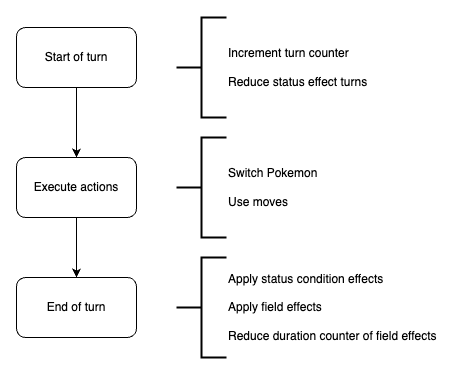
\includegraphics[width=.75\textwidth]{assets/turn-order-of-operations.png}
    \caption{Turn order of operations.}
    \label{fig:turn-order-of-operations}
\end{figure}

Entities with start of turn or end of turn effects expose a \lstinline|on_turn_start| or \lstinline|on_turn_end| function
that can be called inside the step function (see listing \ref{lst:turn-end-func}). This is based on
the Facade design pattern and makes sure the environment doesn't need to know the full details of how each entity needs
to be handled. This approach is also partially inspired by an observer pattern as the relevant entities are "subscribed"
to the start/end of turn events in the environment.
\begin{lstlisting}[language=Python,caption={Example of the environment handling the end of a turn without knowing each entity's full implementation.},float=h,label=lst:turn-end-func,breaklines]
def on_turn_end(self, sorted_active_pokemon: list[Pokemon]):
    for pkm in sorted_active_pokemon:
        pkm.on_turn_end()
    self.state.battle_effects_manager.on_turn_end(sorted_active_pokemon)
\end{lstlisting}

\subsubsection{Move handling}
There are many categories of moves in Pokemon that have to be handled in different ways. In the teambuilder \cite{TeambuilderCli},
move data is gathered together with the Pokemon. We use the data to determine which category a move belongs to and thus how
to handle it. Move handling is defined in the \lstinline|BattleActions| class. If the agent chooses a move as its action
the \lstinline|BattleActions.executeMove| method is called (see listing \ref{lst:exec-move-func}). This method checks the 
move's category and matches it to the appropriate handler to calculate how much damage is dealt, how much health is restored 
and whether or not a secondary effect occurs.

\begin{lstlisting}[basicstyle=\fontsize{10}{10}\selectfont\ttfamily,language=Python,caption={Excerpt of the execute move function.},float=h,label=lst:exec-move-func,breaklines]
def execute_move(self, move: PokemonMove, attacker: Pokemon, target: Pokemon):
    if not self._can_execute_move(attacker, move, target):
        return

    inflicted_damage = 0
    restored_health = 0

    match move.category:
        case 'ailment':
            self._handle_ailment_move(move, target)
        case 'damage':
            inflicted_damage = self._handle_damage_move(move, attacker, target)
        case 'damage+ailment':
            inflicted_damage = self._handle_damage_with_ailment_move(move, attacker, target)
        [...]
        case 'damage+lower' | 'damage+raise':
            inflicted_damage = self._handle_damage_with_stat_change(move, attacker, target)
        case 'damage+heal':
            inflicted_damage = self._handle_damage_with_healing(move, attacker, target)
            restored_health = math.floor(inflicted_damage * (move.drain / 100))
        [...]
        case 'field-effect':
            self._handle_field_effect(move, target)
        case 'unique':
            self._handle_unique_move(move, target)

    self._apply_move_effects(move, attacker, target, inflicted_damage, restored_health)
\end{lstlisting}

Damage is calculated using a close approximation of the official Pokemon damage formula, however due to not implementing 
the full set of Pokemon mechanics it is not entirely faithful and will deviate from reality by a small amount. When comparing
to a fully featured damage calculator the implementation is usually off by 1 or 2 damage points. This may also be caused 
by the alternative rounding rules utilized by the Pokemon games, as the official games round down at 0.5 and it is not well-documented
where exactly rounding occurs in the formula. However, as this deviation is the same for both agents it was deemed to be 
good enough in terms of creating a faithful simulator.
